%---------------------------------------------------------------------------
% Gui component.
%
%---------------------------------------------------------------------------
\section{GUI component}
\label{sec:arch_gui}

Graphical user interfaces are the most commonly used form of interaction with user in modern computing. Designing a decent user interface is especially significant due to the aim of this work - to create a measurement and visualization tool. Although GUI component has a rather limited role of providing the user with control over application and allowing viewing the results of the work, in fact, it is the most complex component. Additionally, any shortcoming in the GUI is relatively difficult to hide from the user. It makes the UI/UX (User Interface/User Experience) engineering crucial.

While designing the user interface, I was trying to follow a few general principles. First of all, I wanted the resulting interface to be as transparent as possible. Users should focus on their tasks instead of learning how to use the tool. Because of that, the application should not be bloated with unnecessary options and steps that the users need to perform to achieve their goals. It should be as concise as possible. Because the measurement visualization is probably the most essential functionality of the application, it needs a significant concern. User should be able to view charts with the results without any interruptions or any other UI components that might be disturbing. What is also noteworthy, the GUI must be coherent to free the user from the chaos of being spread across multiple windows, desktops.

From the business logic point of view, GUI component will extensively use MVC design pattern~\cite{gamma1995}. Each form, window or more complex section needs to have its own view, responsible for presentation, the controller that collects user's events and updates the view on user\rq{}s actions or system events. The application will use a shared model, which will be an access point for the underlying components, external to the GUI.

\subsection{Interface Mockups}

In this section, I will try to describe mockups of the most fundamental views. The first one, depicted in Figure~\ref{fig:mock_main} shows the main application view. The left edge of the application window contains a vertical tab pane controller that allows the user to switch between views covering the most notable application contexts - resources, measurements and visualizations. Another benefit of such an approach is that the application has a lot of space for what the user needs. The second most vital component of the main view is a menu bar placed on the top. It allows a user to perform bulk operations (e.g. pause all measurements) regardless of the view that a user currently sees.

All the subsequent mockups cover context-specific views that application renders in the central pane of the main view.

\begin{figure}[ht]
\centering
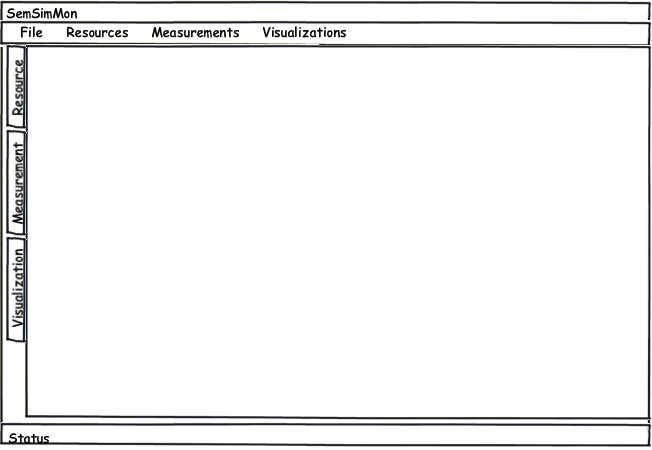
\includegraphics[width=0.7\textwidth]{mock_main}
\caption{GUI application main view mockup}
\label{fig:mock_main}
\end{figure}

When the user starts working with the application, first they must add the resources to measure. Because of that the resources view is the first, initial section displayed directly after a startup. The resources mockup can be found in Figure~\ref{fig:mock_resources}. The view is divided into two high level logical parts - the left pane covers the global resources context - the user can browse the measurement tree as well as add new resources into it. The right pane is specific to a resource selected by user from the tree on left and contains an accordion UI component with two sections. The upper one shows the resource\rq{}s static attributes. The one below allows the user to see snapshot of resource\rq{}s dynamic state and check all its capabilities at a given point of time. It contains also the Refresh button, to allow the user to refresh these values. Additionally, below the accordion there are several buttons allowing performing actions on a selected resource.

\begin{figure}[ht]
\centering
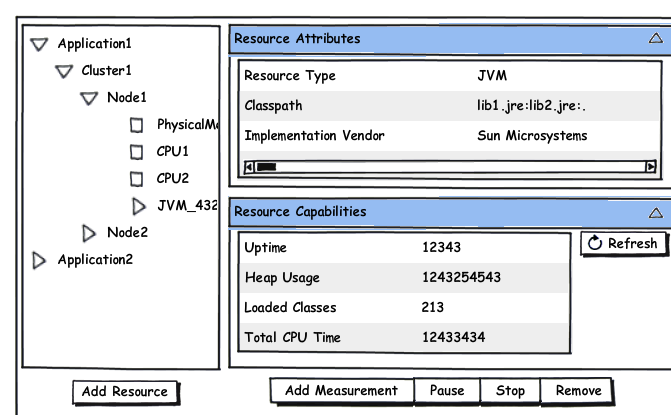
\includegraphics[width=0.7\textwidth]{mock_resources}
\caption{GUI application resources pane}
\label{fig:mock_resources}
\end{figure}

Figure~\ref{fig:mock_measurements} covers the measurements context of the application. All the measurements created are listed on the left side of this view. The accordion on the right side shows details of the selected measurement. The upper section contains a table with a general information. The lower one shows all values gathered since the creation of the selected resource. Using controls under the measurements list, the user can pause, resume or remove the measurement. Additionally in this section the user may copy the results to the clipboard, in CSV format which can be easily imported to any spreadsheet application for a further analysis.

\begin{figure}[ht]
\centering
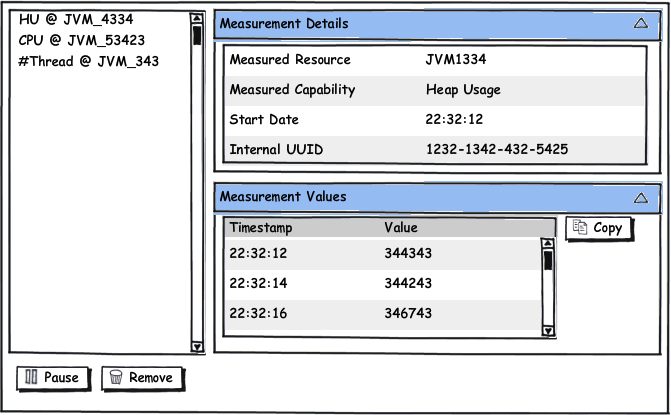
\includegraphics[width=0.7\textwidth]{mock_measurements}
\caption{GUI application measurements pane}
\label{fig:mock_measurements}
\end{figure}

\begin{figure}[ht]
\centering
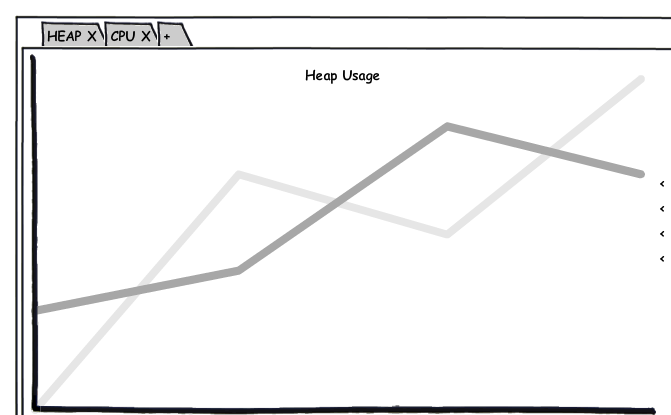
\includegraphics[width=0.7\textwidth]{mock_vis_clean}
\caption{GUI application visualizations pane, a clean view}
\label{fig:mock_vis_clean}
\end{figure}

Appropriate visualization displays are probably the most difficult ones to design, from the user engineering experience perspective. I used some modern web browsers interfaces as an inspiration, when designing this UI component. The effects can be seen in Figure~\ref{fig:mock_vis_clean}. In the proposed solution every visualization is being rendered on a separate, horizontal tab. The user should just click the last tab with prompting a icon to add a new visualization. To remove a visualization, the user simply clicks a cross icon on the visualization\rq{}s tab, just as they would close tab in a browser. This gives a visualization chart as much space as possible and still allows the user to control the creation and disposal of visualization.

Where to place controls of a visualization is the biggest problem with such an approach. The user must be able to choose which measurements should be included in a given visualization, as well as a chart type or define other configuration settings. A management pane was designed to address this need. It is hidden by default and is being displayed to the user, on mouse over the right edge of chart, the one marked with \lq{}<\rq{} signs. Figure~\ref{fig:mock_vis_options} depicts the layout of this pane. The settings pane contains a form, divided into several sections:

\begin{itemize}

\item Visualization Options - here user can configure the label of the whole visualization, as can be seen on the tab pane.

\item Chart Options - allows setting a chart title (the rendered on chart graphics pane) and choose a type of the chart. The user will be able to use a time series (XY scatter), a pie, a bar and a spider web chart types.

\item Measurements - enables control over which measurements should be included in a given visualization. To add a measurement into a visualization, the user should click the \lq\lq{}Add\rq\rq{} button and choose which measurements should be included, from the displayed dialog. The user will be able to remove a given measurement from the chart, by simply selecting it from the list and clicking the Remove button.

\item Actions - allows the user to pause and resume a visualization. Additionally the user can copy to clipboard an image containing a snapshot of the visualization's chart.
\end{itemize}

\begin{figure}[ht]
\centering
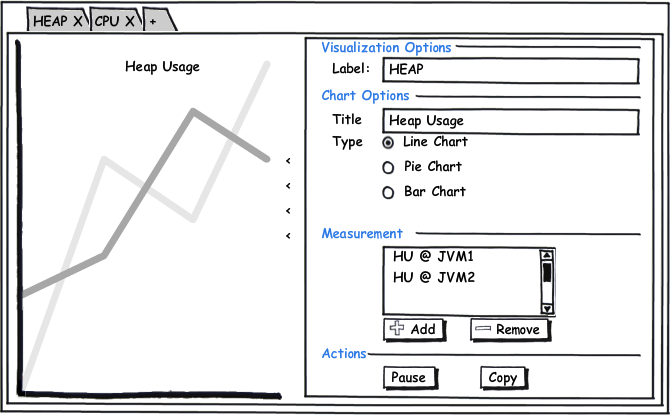
\includegraphics[width=0.7\textwidth]{mock_vis_options}
\caption{GUI application visualizations pane, a view with the options pane}
\label{fig:mock_vis_options}
\end{figure}

